\documentclass[11pt]{article}

\usepackage[margin=0.8in]{geometry}
\usepackage[T1]{fontenc}
\usepackage{lmodern}
\usepackage{booktabs}
\usepackage{graphicx}
\usepackage{hyperref}
\usepackage{pgfplots}
\usepgfplotslibrary{groupplots}
\pgfplotsset{compat=1.18}
\setlength{\emergencystretch}{2em}

\title{Microarchitectural Characterization of Dynamic Language Runtimes\\
\large Checkpoint II: LLC Capacity and Prefetching}
\author{Y Tagore Ravindra Sree}
\date{\today}

\begin{document}
\maketitle

\begin{abstract}
This report extends the earlier Python and Java trace study. It sweeps last-level
cache (LLC) capacity and compares two L1 data-cache prefetchers on pointer
chasing. LLC size did not change cycles in these trace windows. Next-line and
IP-stride prefetching reduced cycles for the Python pointer-chase trace, but
neither helped the Java trace. The results are from ChampSim trace replay, not
execution-time measurements on a real processor.
\end{abstract}

\section{Question}
The first checkpoint found little change when the LLC was enlarged from
2\,MiB to 8\,MiB. This checkpoint tests more LLC sizes to see whether the
measured traces show a capacity point where misses or cycles level off. It also
tests whether simple hardware prefetchers help with dependent pointer loads.

\section{Method}
The experiment reuses the 1,000,000-instruction traces from checkpoint 1.
ChampSim warms up for 100,000 instructions and measures about 899,000. The
LLC sweep tests 0.5, 1, 2, 4, 8, and 16\,MiB. Only LLC capacity changes;
latency remains 20 cycles. The existing 2\,MiB baseline and 8\,MiB results are
reused.

For the pointer-chase traces, the baseline with no prefetching is compared
against \texttt{next\_line} and \texttt{ip\_stride} prefetching at L1D. Python
and Java use the same trace and simulation settings as the LLC sweep. The
reported prefetch usefulness counters come from L1D.

\section{LLC capacity results}
\begin{figure}[htbp]
\centering
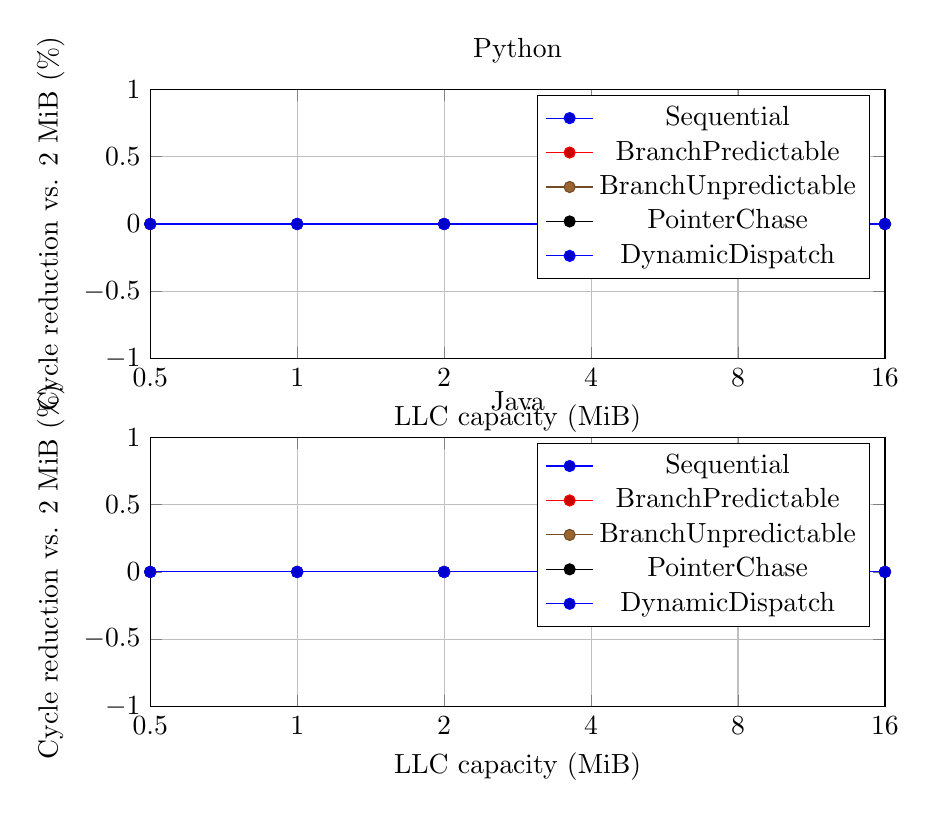
\begin{tikzpicture}
\begin{groupplot}[
  group style={group size=1 by 2,vertical sep=1cm},
  width=0.9\textwidth,height=5cm,
  xmode=log,log basis x=2,xmin=0.5,xmax=16,
  xtick={0.5,1,2,4,8,16},
  xticklabels={$0.5$,$1$,$2$,$4$,$8$,$16$},
  xlabel={LLC capacity (MiB)},
  ylabel={Cycle reduction vs. 2 MiB (\%)},
  ymin=-1.00,ymax=1.00,
  grid=major,
]
\nextgroupplot[title={Python}]
\addplot+[mark=*] coordinates {(0.5,0.00) (1,0.00) (2,0.00) (4,0.00) (8,0.00) (16,0.00)};
\addlegendentry{Sequential}
\addplot+[mark=*] coordinates {(0.5,0.00) (1,0.00) (2,0.00) (4,0.00) (8,0.00) (16,0.00)};
\addlegendentry{BranchPredictable}
\addplot+[mark=*] coordinates {(0.5,0.00) (1,0.00) (2,0.00) (4,0.00) (8,0.00) (16,0.00)};
\addlegendentry{BranchUnpredictable}
\addplot+[mark=*] coordinates {(0.5,0.00) (1,0.00) (2,0.00) (4,0.00) (8,0.00) (16,0.00)};
\addlegendentry{PointerChase}
\addplot+[mark=*] coordinates {(0.5,0.00) (1,0.00) (2,0.00) (4,0.00) (8,0.00) (16,0.00)};
\addlegendentry{DynamicDispatch}
\nextgroupplot[title={Java}]
\addplot+[mark=*] coordinates {(0.5,0.00) (1,0.00) (2,0.00) (4,0.00) (8,0.00) (16,0.00)};
\addlegendentry{Sequential}
\addplot+[mark=*] coordinates {(0.5,0.00) (1,0.00) (2,0.00) (4,0.00) (8,0.00) (16,0.00)};
\addlegendentry{BranchPredictable}
\addplot+[mark=*] coordinates {(0.5,0.00) (1,0.00) (2,0.00) (4,0.00) (8,0.00) (16,0.00)};
\addlegendentry{BranchUnpredictable}
\addplot+[mark=*] coordinates {(0.5,0.00) (1,0.00) (2,0.00) (4,0.00) (8,0.00) (16,0.00)};
\addlegendentry{PointerChase}
\addplot+[mark=*] coordinates {(0.5,0.00) (1,0.00) (2,0.00) (4,0.00) (8,0.00) (16,0.00)};
\addlegendentry{DynamicDispatch}
\end{groupplot}
\end{tikzpicture}
\caption{Cycle change across the LLC capacity sweep. Positive values indicate fewer cycles than the 2 MiB run.}
\end{figure}
\begin{figure}[htbp]
\centering
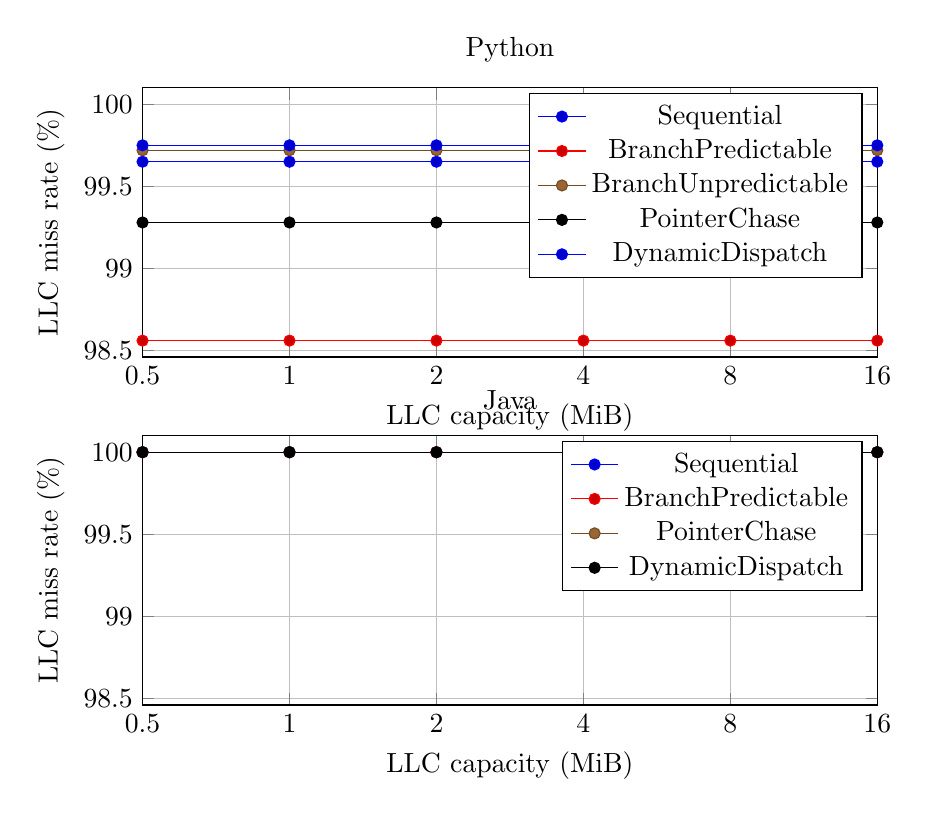
\begin{tikzpicture}
\begin{groupplot}[
  group style={group size=1 by 2,vertical sep=1cm},
  width=0.9\textwidth,height=5cm,
  xmode=log,log basis x=2,xmin=0.5,xmax=16,
  xtick={0.5,1,2,4,8,16},
  xticklabels={$0.5$,$1$,$2$,$4$,$8$,$16$},
  xlabel={LLC capacity (MiB)},
  ylabel={LLC miss rate (\%)},
  ymin=98.46,ymax=100.10,
  grid=major,
]
\nextgroupplot[title={Python}]
\addplot+[mark=*] coordinates {(0.5,99.65) (1,99.65) (2,99.65) (4,99.65) (8,99.65) (16,99.65)};
\addlegendentry{Sequential}
\addplot+[mark=*] coordinates {(0.5,98.56) (1,98.56) (2,98.56) (4,98.56) (8,98.56) (16,98.56)};
\addlegendentry{BranchPredictable}
\addplot+[mark=*] coordinates {(0.5,99.72) (1,99.72) (2,99.72) (4,99.72) (8,99.72) (16,99.72)};
\addlegendentry{BranchUnpredictable}
\addplot+[mark=*] coordinates {(0.5,99.28) (1,99.28) (2,99.28) (4,99.28) (8,99.28) (16,99.28)};
\addlegendentry{PointerChase}
\addplot+[mark=*] coordinates {(0.5,99.75) (1,99.75) (2,99.75) (4,99.75) (8,99.75) (16,99.75)};
\addlegendentry{DynamicDispatch}
\nextgroupplot[title={Java}]
\addplot+[mark=*] coordinates {(0.5,100.00) (1,100.00) (2,100.00) (4,100.00) (8,100.00) (16,100.00)};
\addlegendentry{Sequential}
\addplot+[mark=*] coordinates {(0.5,100.00) (1,100.00) (2,100.00) (4,100.00) (8,100.00) (16,100.00)};
\addlegendentry{BranchPredictable}
\addplot+[mark=*] coordinates {(0.5,100.00) (1,100.00) (2,100.00) (4,100.00) (8,100.00) (16,100.00)};
\addlegendentry{PointerChase}
\addplot+[mark=*] coordinates {(0.5,100.00) (1,100.00) (2,100.00) (4,100.00) (8,100.00) (16,100.00)};
\addlegendentry{DynamicDispatch}
\end{groupplot}
\end{tikzpicture}
\caption{LLC miss rate across the tested capacities. Java BranchUnpredictable has no LLC accesses and is omitted.}
\end{figure}


The CSV file \texttt{checkpoint2\_llc\_sweep.csv} contains IPC, cycles, memory
wait share, and L1D and LLC miss counts for every run. A capacity knee in these
plots is only an effective threshold for these trace windows and this
simulator configuration. In these runs, all six capacities produced the same
cycles and miss counts for each workload. Where there were LLC accesses, the
LLC miss rate stayed between 98.56\% and 100\%. The Java unpredictable-branch
trace had no LLC accesses, so its LLC miss rate is not defined. There is no
capacity knee in the tested 0.5--16\,MiB range, so these results cannot locate
a working-set threshold. The flat curve could mean little reuse in the captured
window or a footprint beyond the tested range.

\section{Pointer-chase prefetch results}
\begin{table}[htbp]
\centering
\small
\resizebox{\textwidth}{!}{%
\begin{tabular}{llrrrrrrr}
\toprule
Runtime & L1D prefetcher & IPC & Cycles & Cycle reduction (\%) & Memory wait (\%) & L1D miss (\%) & LLC miss (\%) & Useful / issued \\
\midrule
Python & None & 0.9899 & 908178 & +0.00 & 47.96 & 4.39 & 99.28 & 0/0 \\
Python & Next-line & 1.1110 & 809460 & +10.87 & 41.29 & 3.88 & 98.66 & 1845/171248 \\
Python & IP-stride & 1.0330 & 870068 & +4.20 & 45.43 & 3.15 & 99.13 & 849/38373 \\
Java & None & 0.8578 & 1048083 & +0.00 & 75.46 & 2.04 & 100.00 & 0/0 \\
Java & Next-line & 0.8400 & 1070226 & -2.11 & 75.44 & 1.42 & 99.51 & 80/270309 \\
Java & IP-stride & 0.8578 & 1048085 & +0.00 & 75.46 & 2.04 & 100.00 & 0/102 \\
\bottomrule
\end{tabular}%
}
\caption{Pointer-chase results. Prefetch usefulness counts are from the L1D.}
\end{table}


Prefetches can be issued without helping. The useful and issued counts should
be read alongside the cycle change and miss rates. These counters describe the
simulator's L1D prefetch behavior; they are not measurements of a commercial
processor.

For Python, next-line prefetching reduced cycles from 908,178 to 809,460
(10.87\%). IP-stride reduced them to 870,068 (4.20\%). The memory-wait share
fell from 47.96\% to 41.29\% with next-line and 45.43\% with IP-stride.
For Java, next-line increased cycles from 1,048,083 to 1,070,226 (2.11\%).
IP-stride changed the count by only two cycles. Java's memory-wait share
remained about 75.46\%. The prefetcher counters show that only a small fraction
of issued prefetches were useful, especially for Java.

This suggests next-line prefetching is worth testing further on the Python
trace, but it does not show that it will help Python programs generally. Neither
prefetcher solved the Java pointer-chase bottleneck in this trace. Increasing
LLC capacity also gave no benefit in the tested range. A better next experiment
would use longer or repeated trace windows and a workload with known LLC reuse.

\section{Interpretation and limits}
The LLC sweep and prefetcher comparison replay a single trace window per
workload and language. There are no repeated runs to measure variation.
Interpreter and JVM instructions are included, and the Python and Java data
layouts are not identical. A flat miss-rate or cycle curve means that the
tested trace did not benefit measurably from those configurations; it does not
show that cache capacity or prefetching is unimportant in general.

\subsection{Takeaway}
The strongest result is the difference between the two pointer-chase traces:
the Python trace benefited from both tested prefetchers, while the Java trace
did not. LLC capacity from 0.5 to 16\,MiB made no measurable difference for any
of the ten workload traces. These results are clues about the captured windows,
not a ranking of the languages or a general hardware recommendation.

\section{Reproducibility}
In WSL, run:
\begin{verbatim}
bash analysis/run_checkpoint2.sh
python3 analysis/summarize_checkpoint2.py
pdflatex -interaction=nonstopmode -halt-on-error checkpoint2_report.tex
\end{verbatim}
The runner uses existing traces, writes ChampSim output under
\texttt{results/checkpoint2/}, and restores the baseline ChampSim configuration
when it exits. The summary script generates the CSV files, plot source, and
prefetch table used here.

\end{document}
